\documentclass[10pt]{article}
\usepackage[margin=0.55in,top=0.5in,bottom=0.5in]{geometry}
\usepackage[all]{xy}
\usepackage{caption}
\usepackage{amsmath,amsthm,amssymb,color,latexsym}
\usepackage{mathtools}
\usepackage{geometry}
\usepackage{booktabs}
\geometry{letterpaper}    
\usepackage{graphicx}
\usepackage{tabto}
\usepackage{setspace}
\usepackage[dvipsnames]{xcolor}

\usepackage[noframe]{showframe}
\usepackage{framed}


\renewenvironment{shaded}{%
  \def\FrameCommand{\fboxsep=\FrameSep \colorbox{shadecolor}}%
  \MakeFramed{\advance\hsize-\width \FrameRestore\FrameRestore}}%
 {\endMakeFramed}
\definecolor{shadecolor}{gray}{0.90}

\newtheorem{problem}{Problem}

\newenvironment{solution}[1][\it{Solution:}]{\textbf{#1 } }

\singlespacing

\begin{document}
\graphicspath{{../figures/}{figures/}{332Project2/figures/}}

\begin{titlepage}
   \begin{center}
       \vspace*{9cm}

       \textbf{CS 332 Fall 2025}

       \vspace{0.5cm}
        Project \#1
        \vfill

       \textbf{Koshi Harashima, Ben Cole}\\
       Due Date: 10/22, 2025
            
   \end{center}
\end{titlepage}

\pagebreak

%%%%%%%%%%%%%%%%%%%%%%%%%%%%%%%%%%%%%%%%%%%%%%%%%%%%%%%%%%%
%%%%%%%%%%%%%%%%%%%%%%%% Problems %%%%%%%%%%%%%%%%%%%%%%%%%
%%%%%%%%%%%%%%%%%%%%%%%%%%%%%%%%%%%%%%%%%%%%%%%%%%%%%%%%%%%

%--------------------------------------------------------
\section{Part 1 - A}
\begin{shaded}
\textbf{Methods}\\
In the Adversarial Fair Payoffs (AFP) setting, each round’s payoff is given to the arm with the lowest total reward so far, creating an adversarial environment.  
We simulate $k=3$, $n=1000$ with learning rates $\epsilon=\{0.01, \sqrt{\log k/n}, 100\}$.

\textbf{Results}\\
FTL’s regret grows linearly with rounds, while random and theoretical learning rates keep regret near zero and remain within the analytical bound.  
Total payoffs confirm the same pattern.

\textbf{Takeaways}\\
In adversarial, unpredictable environments, aggressive exploitation (FTL) performs poorly.  
Stable or random learning rates achieve low regret.
\end{shaded}

\section{Part 1 - B}
\begin{shaded}
\textbf{Methods}\\
In the Bernoulli Payoffs (BP) setting, each arm’s reward follows $v_j^i \sim B(p_j)$ with fixed probabilities $p_j$.  
We simulate $k=3$, $n=1000$ under full information.

\textbf{Results}\\
FTL rapidly identifies the best arm and achieves low regret as $n$ increases.  
Random and theoretical learning rates fluctuate around higher regret levels.

\textbf{Takeaways}\\
When payoffs are stationary and one arm is truly optimal, FTL converges efficiently.  
Exploration offers no benefit in stable environments.
\end{shaded}

\section{Part 2 - C}
\begin{shaded}
\textbf{Methods}\\
We apply the Exponential Weights (EW) algorithm to real-world Pachinko data, treating each store as an ``arm.''  
Daily ROI (Return on Investment) is normalized to $[0,1]$, capturing store-level profitability under full information.

\textbf{Model}\\
Tokyo Pachinko stores are compared across days.  
Payoffs are nonstationary since stores adjust machine settings strategically to attract players.

\textbf{Results}\\
FTL quickly identifies and sticks to the best store, causing regret to converge to near zero. Random and theoretical learning rates fail to adapt to shifting ROI patterns and perform worse.

\textbf{Takeaways}\\
Even with noisy real-world data, simple FTL behavior is effective in our sample because the best store tends to persist long enough to be exploited, despite day-to-day noise
\end{shaded}

\section{Part 2 - D}
\begin{shaded}
\textbf{Methods}\\
We build a randomized \emph{Research Payoffs (RP)} model with clusters (correlated papers) and regime shifts.
At round $t$, the agent allocates $w_t\in\Delta^N$ and receives $U_t=\alpha_t^\top w_t$.

\textbf{Model}\\
One cluster is high, one middle, others low; a hidden Markov state switches the dominant cluster with persistence $p$.

\textbf{Algorithms}\\
FTL (past leader), Uniform (even split), and EW/EG ($w_{t+1,i}\propto w_{t,i}e^{\varepsilon \alpha_{t,i}}$).

\textbf{Results}\\
FTL suffers spikes after switches; Uniform has steady underperformance; EW/EG (moderate $\varepsilon$) tracks the dominant cluster and achieves the lowest regret and highest average payoff.

\textbf{Takeaways}\\
Correlation + regime changes break both FTL and Uniform; multiplicative updates with a conservative but nonzero learning rate are robust.
\end{shaded}


\section*{Figures (Compact)}
\vspace{-0.3em}
\noindent\small Note: AFP/BP use $k{=}3,n{=}1000,h{=}1$. Bound: $2h\sqrt{n\log k}\approx110$.

% Row 1: A (AFP)
\begin{figure}[h!]
\centering
\begin{minipage}[t]{0.48\textwidth}
    \centering
    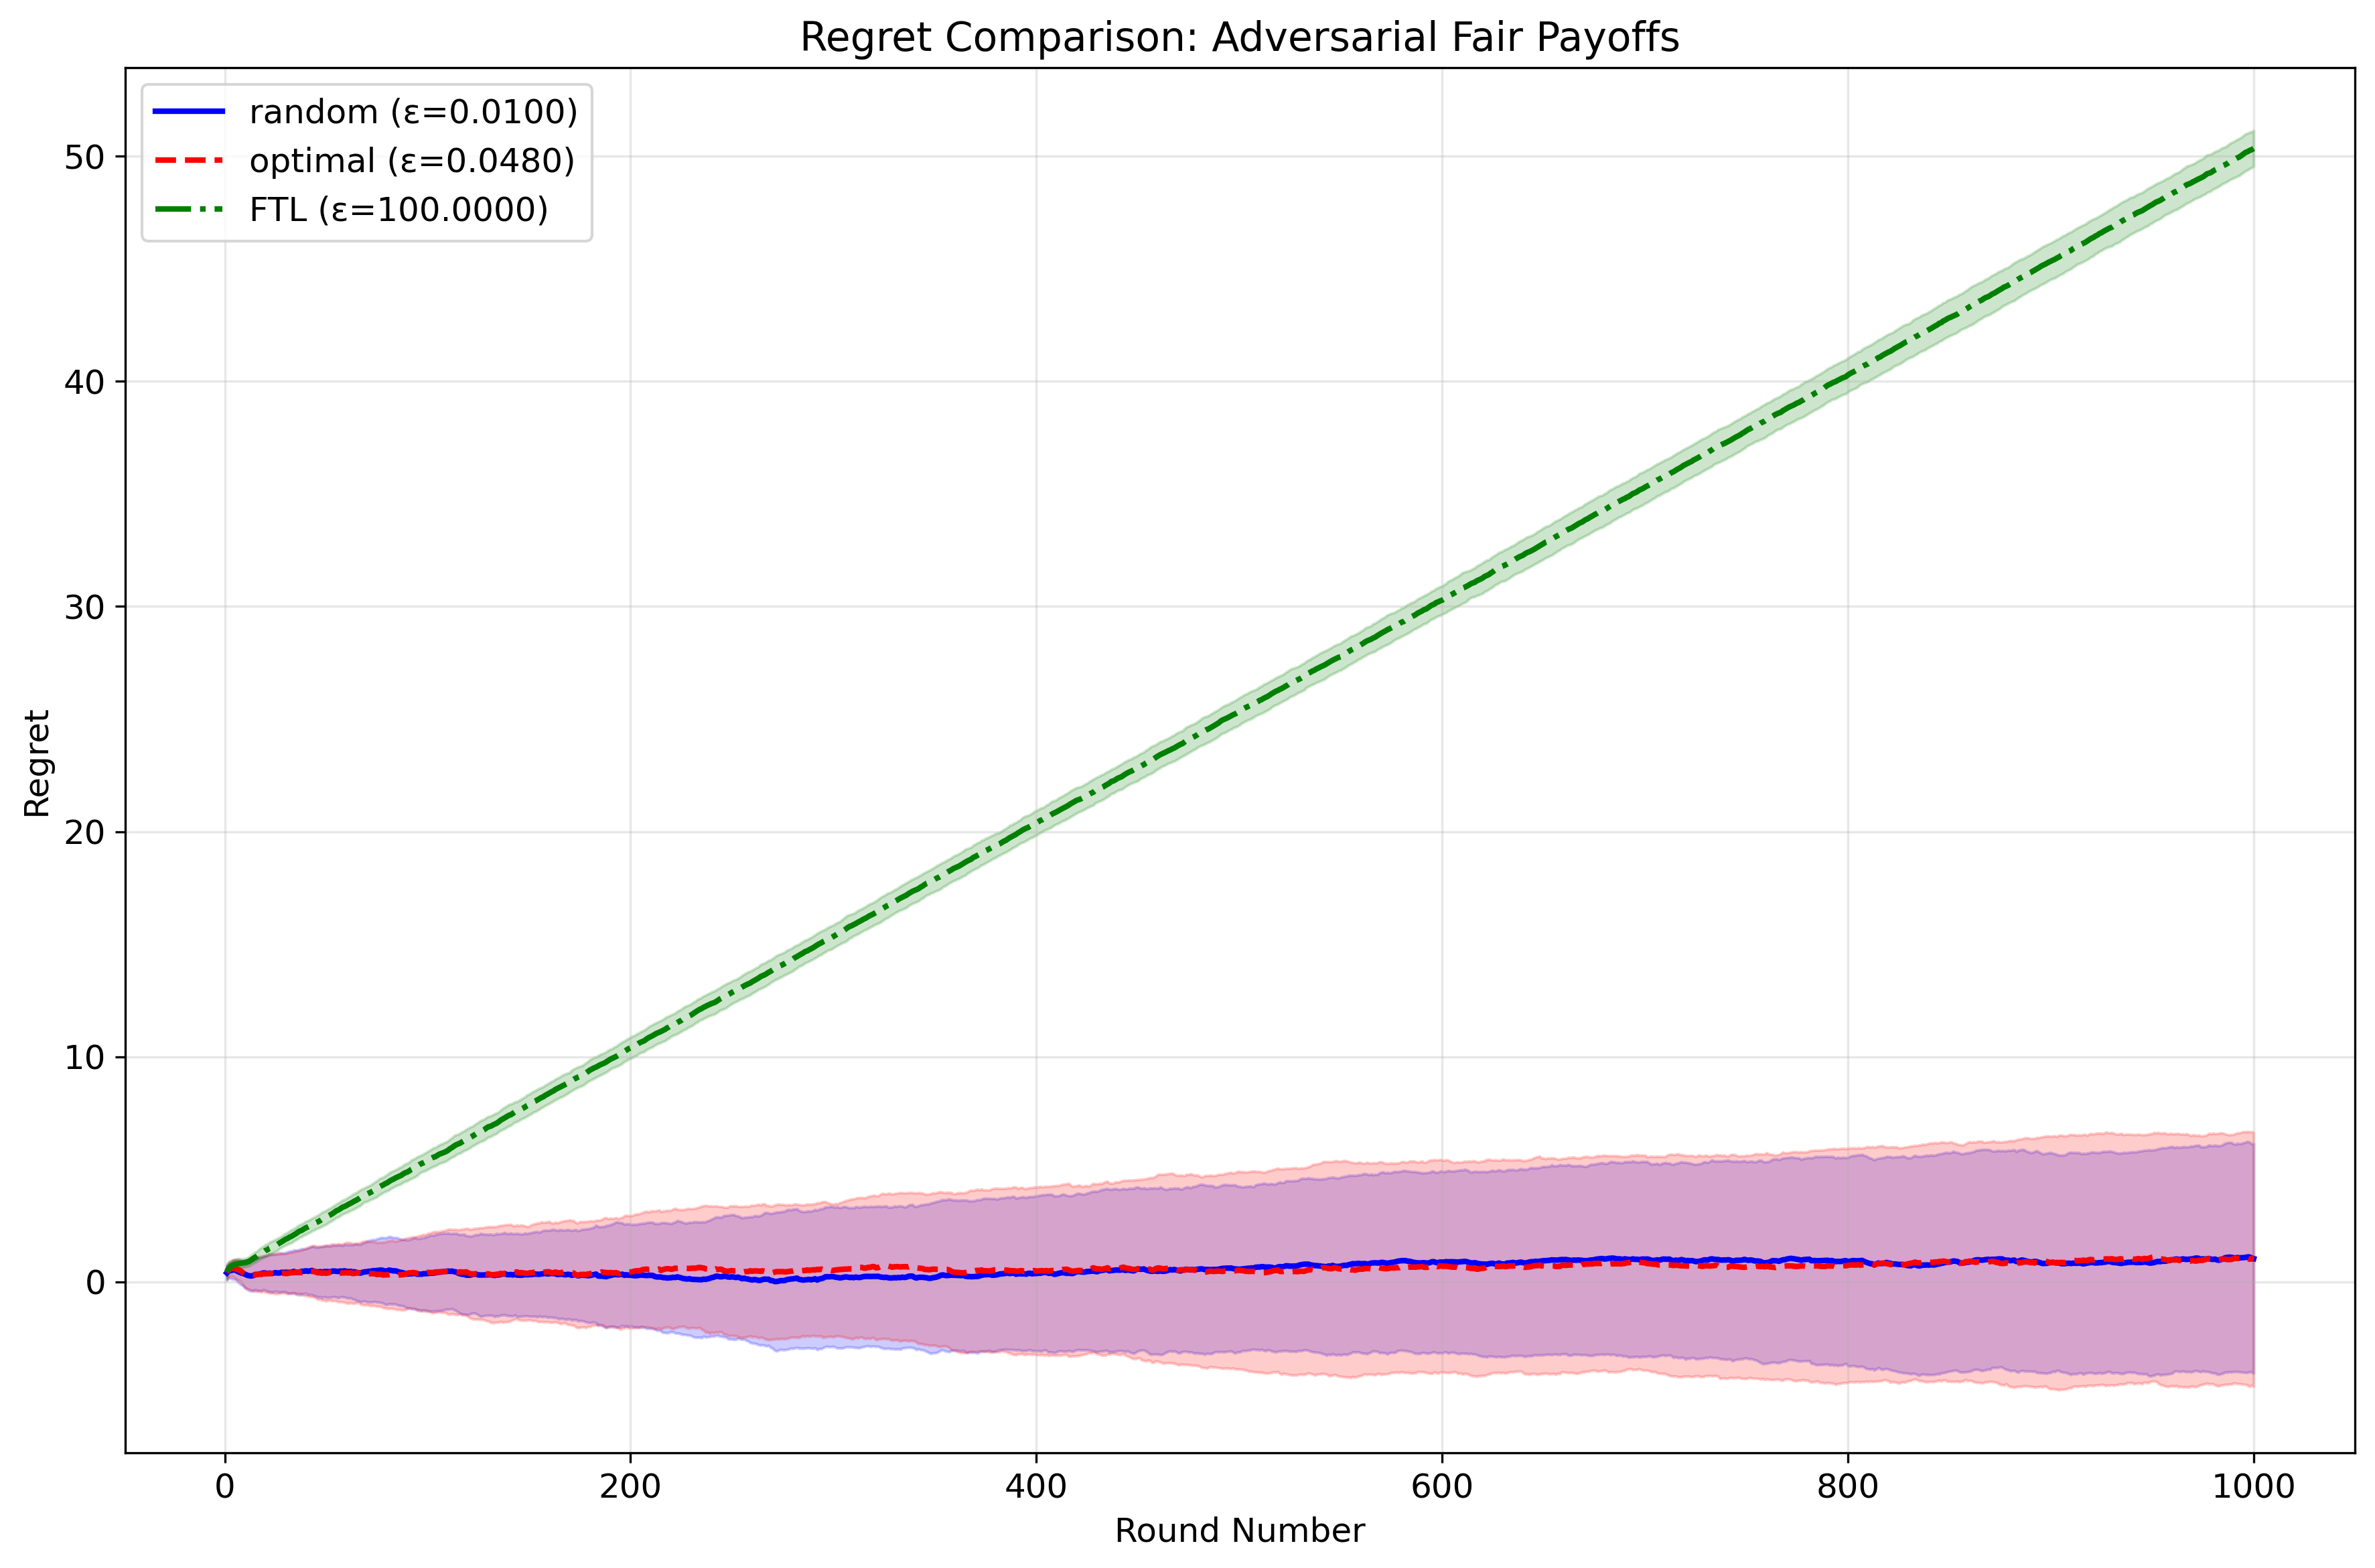
\includegraphics[width=\linewidth]{adversarial_regret_comparison.png}
    \caption*{\footnotesize A: Regret vs.\ rounds}
\end{minipage}\hfill
\begin{minipage}[t]{0.48\textwidth}
    \centering
    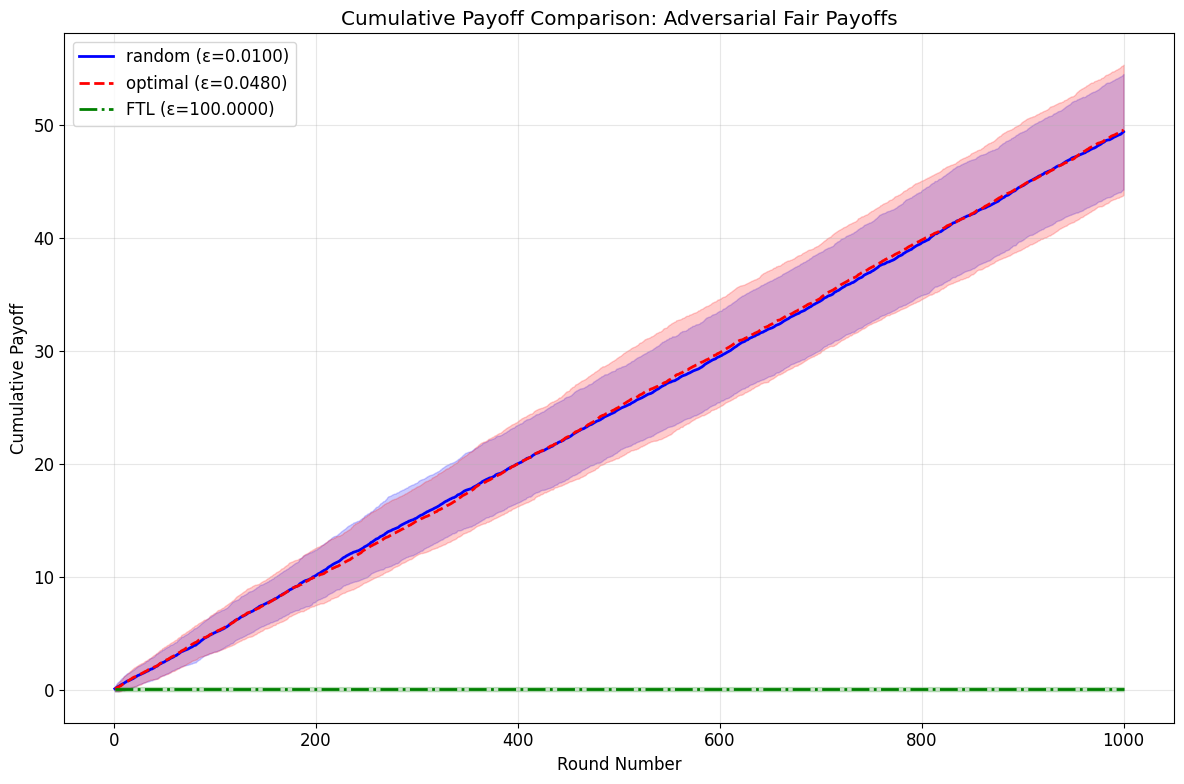
\includegraphics[width=\linewidth]{AFR_payoff.png}
    \caption*{\footnotesize A: Total payoff}
\end{minipage}
\end{figure}

% Row 2: B (BP)
\begin{figure}[h!]
\centering
\begin{minipage}[t]{0.48\textwidth}
    \centering
    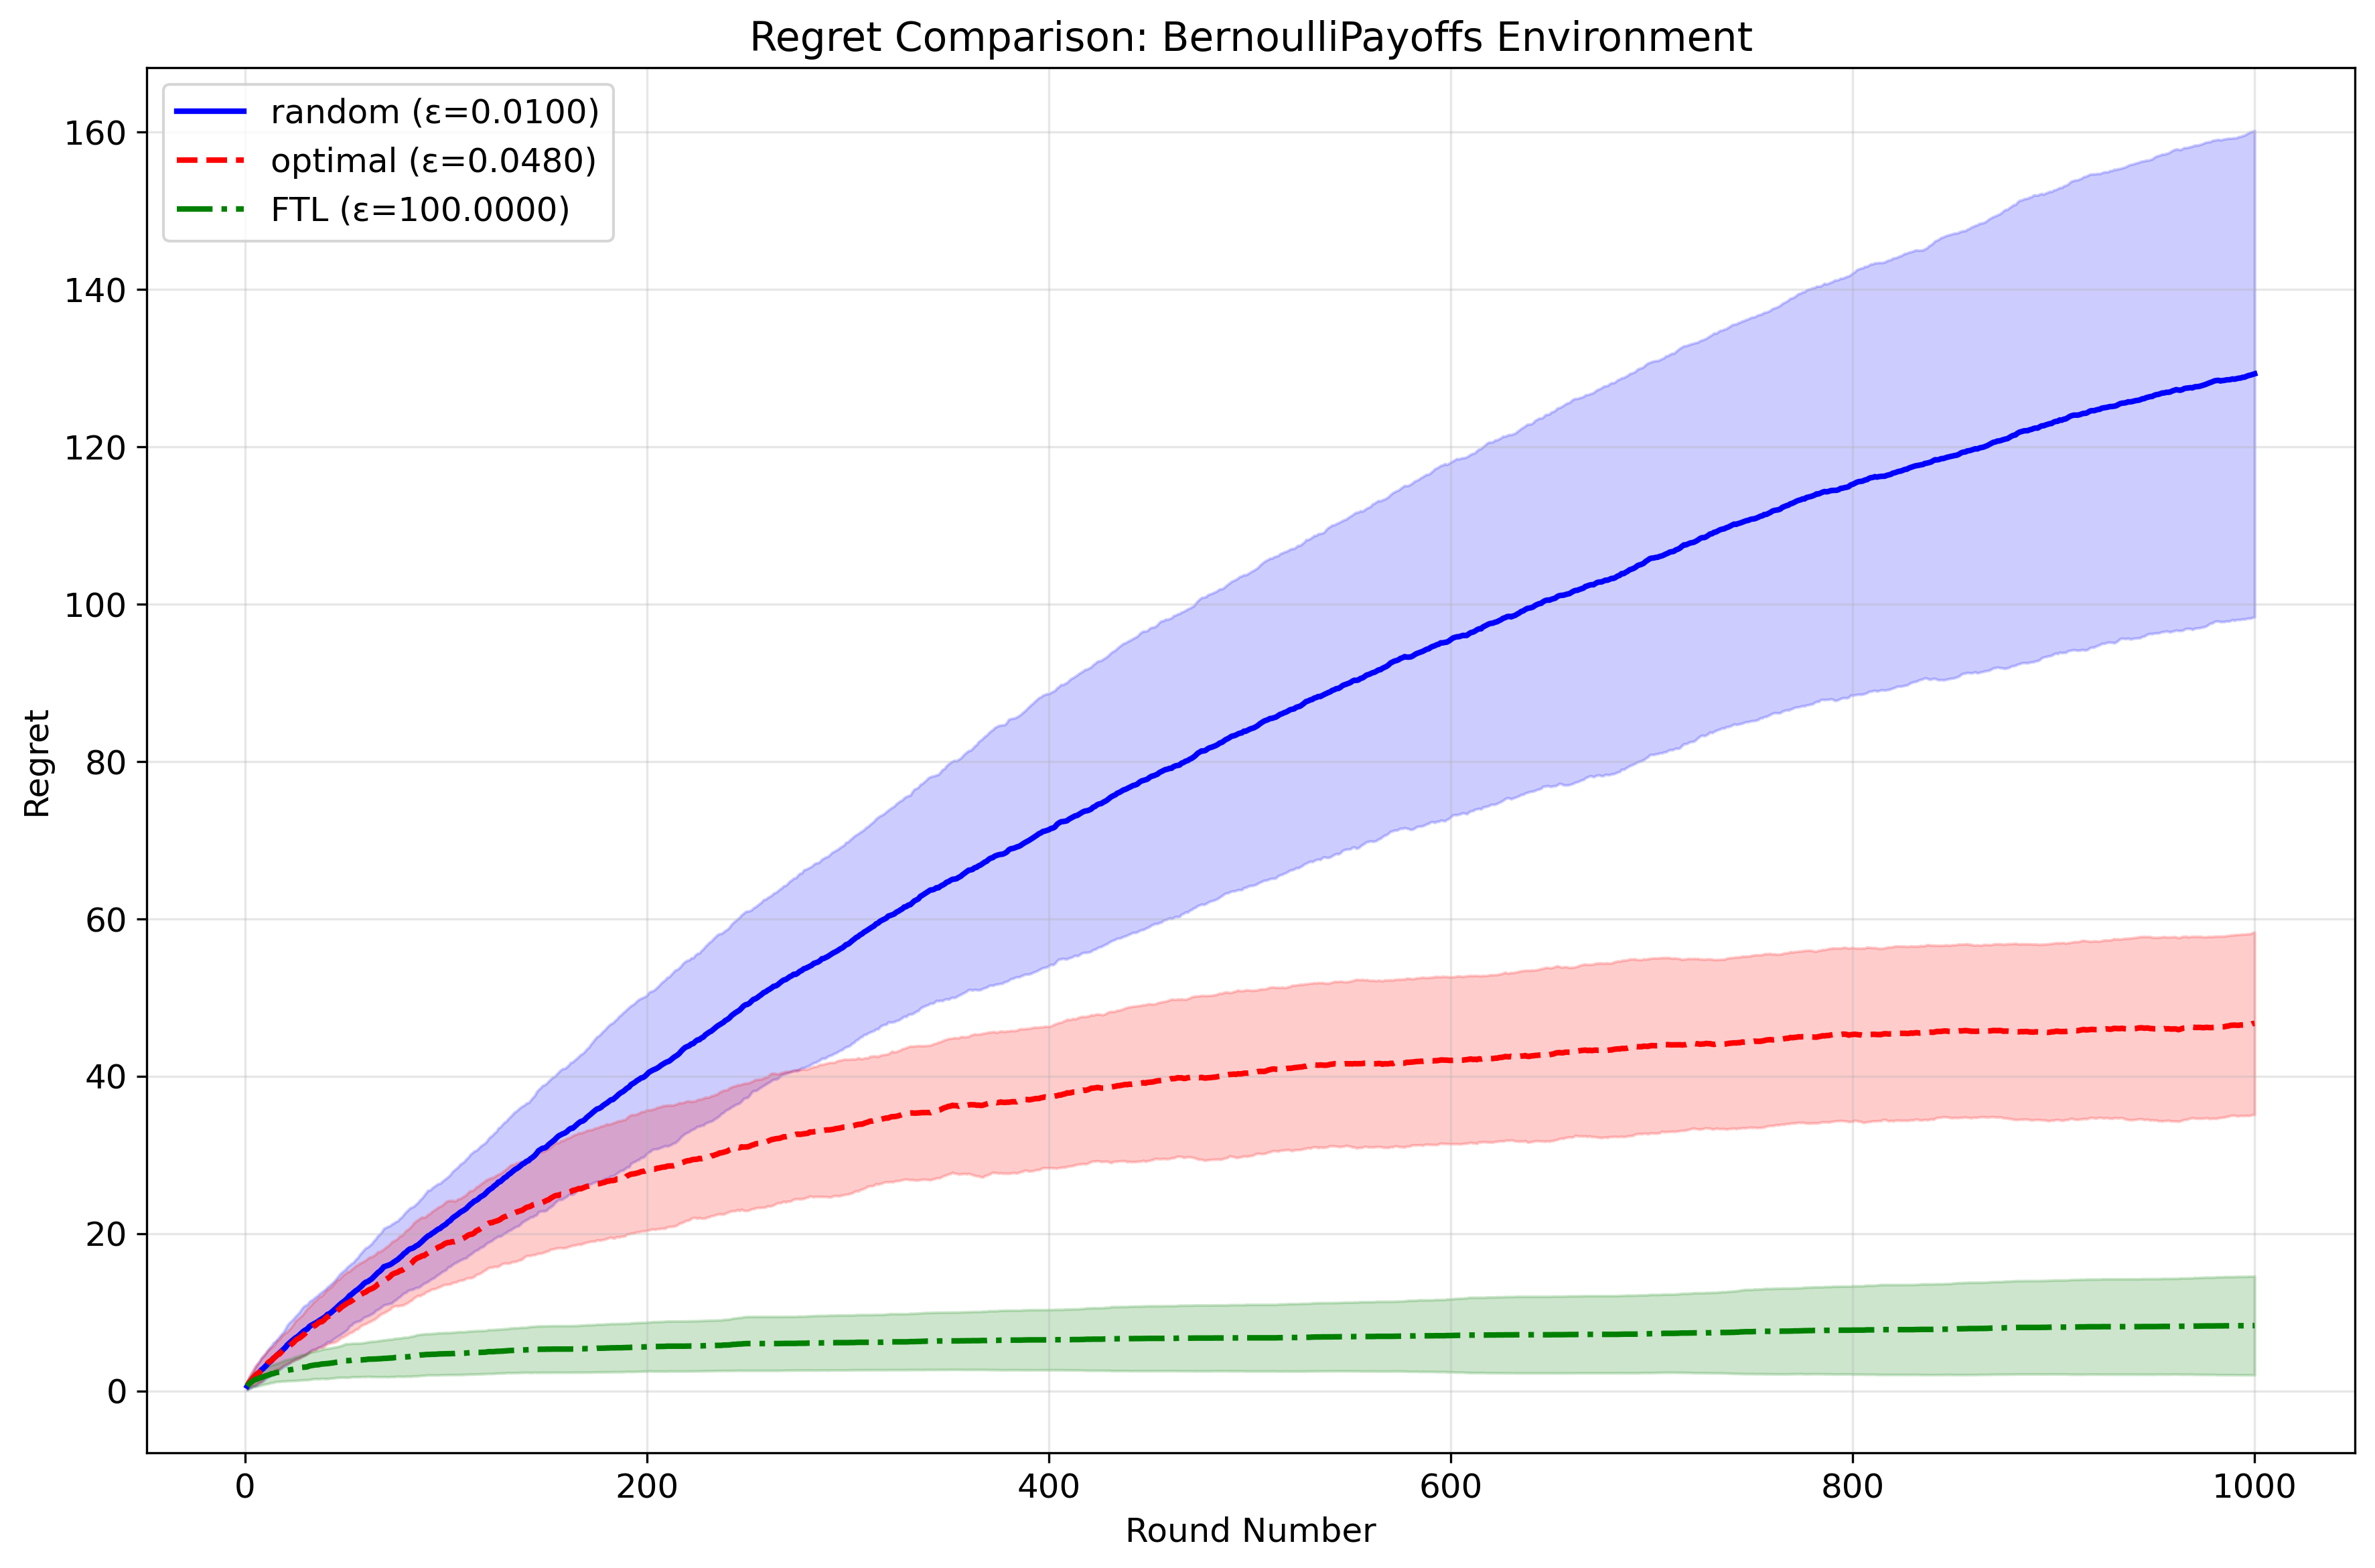
\includegraphics[width=\linewidth]{bernoulli_regret_comparison.png}
    \caption*{\footnotesize B: Regret vs.\ rounds}
\end{minipage}\hfill
\begin{minipage}[t]{0.48\textwidth}
    \centering
    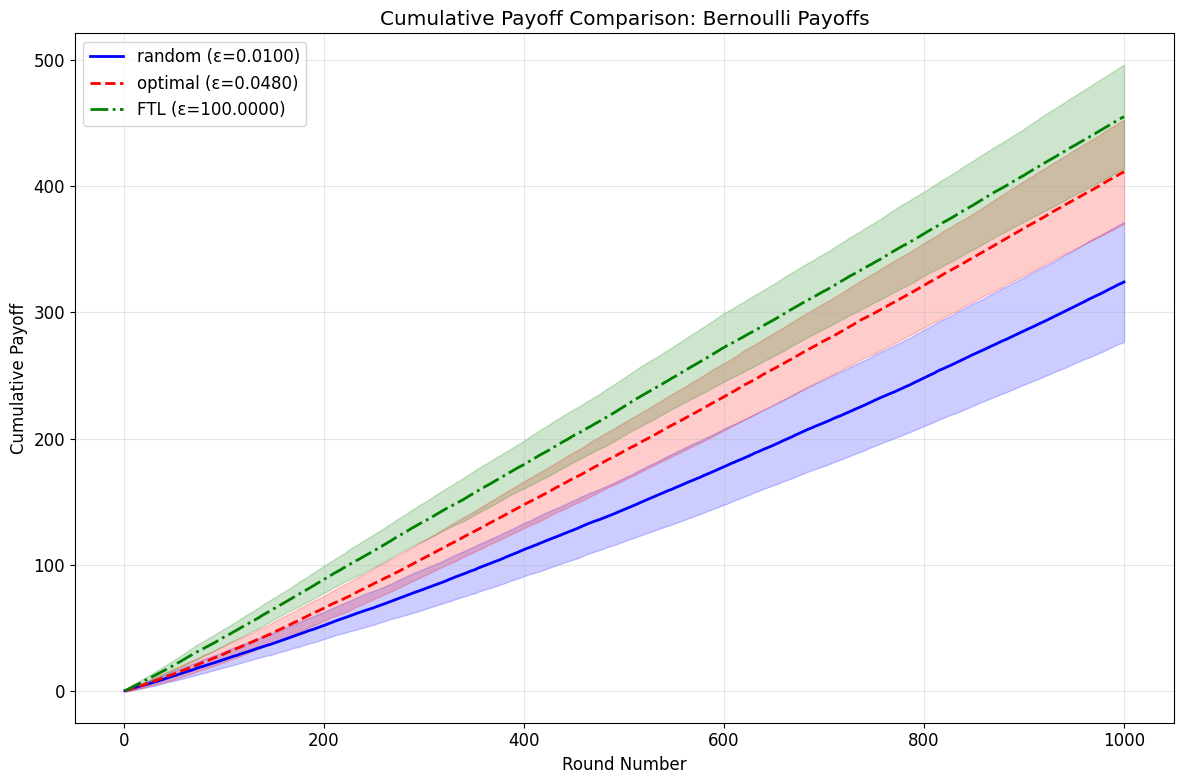
\includegraphics[width=\linewidth]{BP_payoff.png}
    \caption*{\footnotesize B: Total payoff}
\end{minipage}
\end{figure}

% Row 3: C (PP) and D (RP)
\begin{figure}[h!]
\centering
\begin{minipage}[t]{0.48\textwidth}
    \centering
    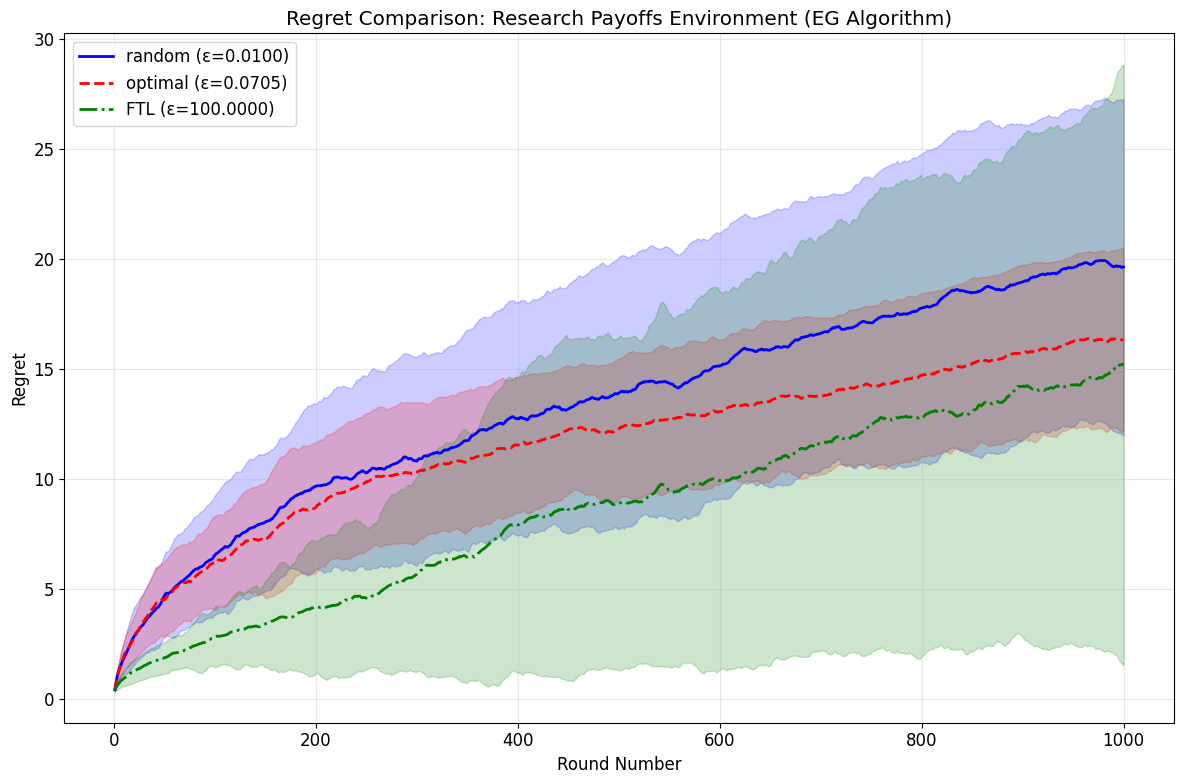
\includegraphics[width=\linewidth]{RP_regret.png}
    \caption*{\footnotesize D: RP regret (regime shifts)}
\end{minipage}
\end{figure}


\end{document}